\begin{pastexam}[label={px:ust-111-ee-ds-10}]{臺聯大電機類 111 學年度 第 10 題}
（追蹤）

(10\%) Binary search trees (BSTs)
\begin{enumerate}[label=(\alph*\,)]
\item What is the resulting BST from successively inserting the keys 7, 3, 6, 9, 8, 4, 2 into an
initially empty tree?
\item What will be the resulting BST after we delete key 3 in the BST in (a)?
\end{enumerate}
\end{pastexam}

\begin{pastsoln}
\textbf{(a)} 每個鍵從根往下比，小的往左、大的往右，走到空的位置就放下（資結書第~9.2~節）。
7 當根；3 放在 7 的左邊；6：$< 7$、$> 3$，放在 3 的右邊；9 放在 7 的右邊；8：$> 7$、$< 9$，放在 9 的
左邊；4：$< 7$、$> 3$、$< 6$，放在 6 的左邊；2：$< 7$、$< 3$，放在 3 的左邊。
\begin{center}
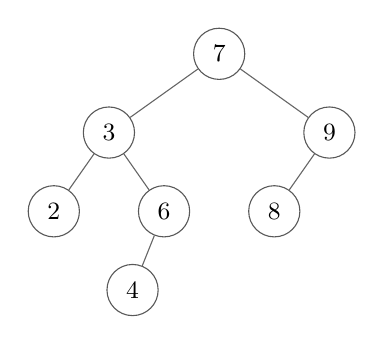
\begin{tikzpicture}[
    btn/.style={circle, draw=black!65, line width=0.4pt, minimum size=6.5mm, inner sep=0pt, font=\small},
    level distance=10mm, edge from parent/.style={draw=black!60},
    level 1/.style={sibling distance=28mm}, level 2/.style={sibling distance=14mm},
    level 3/.style={sibling distance=8mm}]
\node[btn] {7}
    child {node[btn] {3}
        child {node[btn] {2}}
        child {node[btn] {6} child {node[btn] {4}} child[missing]}}
    child {node[btn] {9}
        child {node[btn] {8}}
        child[missing]};
\end{tikzpicture}
\end{center}
檢查：中序是 $2, 3, 4, 6, 7, 8, 9$。

\textbf{(b)} 3 有兩個子節點，照資結書虛擬碼~9.7，用它的\textbf{後繼}（右子樹裡最小的鍵）取代：3 的右子樹
是 $6(4, \cdot)$，最小的是 4。 把 4 的值放到 3 的位置，再從右子樹刪掉 4；4 是葉子，直接拿掉。
\begin{center}
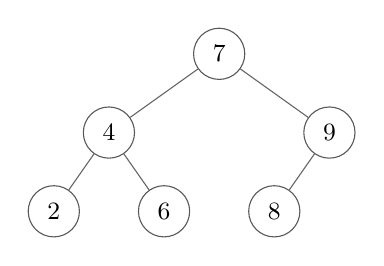
\begin{tikzpicture}[
    btn/.style={circle, draw=black!65, line width=0.4pt, minimum size=6.5mm, inner sep=0pt, font=\small},
    level distance=10mm, edge from parent/.style={draw=black!60},
    level 1/.style={sibling distance=28mm}, level 2/.style={sibling distance=14mm}]
\node[btn] {7}
    child {node[btn] {4}
        child {node[btn] {2}}
        child {node[btn] {6}}}
    child {node[btn] {9}
        child {node[btn] {8}}
        child[missing]};
\end{tikzpicture}
\end{center}
中序是 $2, 4, 6, 7, 8, 9$，仍然是二元搜尋樹。

若改用\textbf{前驅}（左子樹裡最大的鍵）取代，3 的左子樹只有 2，結果是 2 取代 3：
$7\bigl(2(\cdot, 6(4, \cdot)), 9(8, \cdot)\bigr)$，也是正確的刪除。 作答時寫清楚用哪一種。
\end{pastsoln}
